\documentclass[prd,preprintnumbers,twocolumn,eqsecnum,floatfix,letter]{revtex4}
\usepackage{color}
\usepackage{calc}
\usepackage{amsmath,amssymb,graphicx}
\usepackage{amssymb,amsmath}
\usepackage{tensor}
\usepackage{bm}
\usepackage{times}
\usepackage[varg]{txfonts}
\usepackage[colorlinks, pdfborder={0 0 0}]{hyperref}
\definecolor{LinkColor}{rgb}{0.75, 0, 0}
\definecolor{CiteColor}{rgb}{0, 0.5, 0.5}
\definecolor{UrlColor}{rgb}{0, 0, 0.75}
\hypersetup{linkcolor=LinkColor}
\hypersetup{citecolor=CiteColor}
\hypersetup{urlcolor=UrlColor}
\maxdeadcycles=1000
\allowdisplaybreaks
\textwidth 7.5 in 
\hoffset -1 cm 
\newcommand{\comment}[1]{\textcolor{blue}{\textit{#1}}}
\newcommand{\ashok}[1]{\textcolor{red}{\textit{Ashok:#1}}}
\newcommand{\sean}[1]{\textcolor{cyan}{\textit{Sean:#1}}}


\begin{document}

\newcommand{\be}{\begin{equation}}
\newcommand{\ee}{\end{equation}}
\newcommand{\ber}{\begin{eqnarray}}
\newcommand{\eer}{\end{eqnarray}}
\def\bea{\begin{eqnarray}}
\def\eea{\end{eqnarray}}
\newcommand{\etal}{\emph{et al.}}

\newcommand{\Sl}{S_\ell}
\newcommand{\Sigmal}{\Sigma_\ell}
\newcommand{\Flux}{\mathcal{F}}
\newcommand{\LNh}{\hat{\mathbf{L}}_N}
\newcommand{\LN}{\mathbf{L}_N}
\newcommand{\bS}{\mathbf{S}}
\newcommand{\bJ}{\mathbf{J}}
\newcommand{\e}{\mathrm{e}}
\newcommand{\rmi}{\mathrm{i}}
\newcommand{\flow}{f_\mathrm{low}}
\newcommand{\fcut}{f_\mathrm{cut}}

\newcommand{\bchi}{\bm{\chi}}
\newcommand{\blambda}{\bm{\lambda}}
\newcommand{\bLambda}{\bm{\Lambda}}
\newcommand{\bchia}{\bm{\chi}_a}
\newcommand{\bchis}{\bm{\chi}_s}
\newcommand{\chis}{\chi_s}
%\newcommand{\bchi}{\mathbf{\chi}}
\newcommand{\chia}{\chi_a}
\newcommand{\chiadL}{\bchia \cdot \LNh}
\newcommand{\chisdL}{\bchis \cdot \LNh}
\newcommand{\chisSqr}{\bchis^2}
\newcommand{\chiaSqr}{\bchia^2}
\newcommand{\chisDchia}{\bchis \cdot \bchia}
\newcommand{\cA}{\mathcal{A}}
\newcommand{\cB}{\mathcal{B}}
\newcommand{\cC}{\mathcal{C}}
\newcommand{\cP}{\mathcal{P}}
\newcommand{\pc}{{+,\times}}

\title{Spin effect on Christodoulou memory for merging blackhole binaries}
\author{Ashok Choudhary}\email{aschoudhary@mix.wvu.edu}
\author{Sean T. McWilliams}\email{sean.mcwilliams@mail.wvu.edu}
\affiliation{Department of Physics and Astronomy, West Virginia University, Morgantown, WV 26506, USA}


\begin{abstract}
	The Christodoulou memory, which is a nonlinear memory effect sourced by the gravitational wave stress tensor, produce a growing, nonoscillatory change in the gravitational wave "plus" polarization. This results in the permanent displacement of a pair of freely falling test masses after the gravitational wave has passed. While the memory contribution during early in-spiral is well described by Post-Newtonian approximation, the contribution at merger must be obtained from Numerical relativity simulations. The Post-Newtonian corrections upto 3PN order to the gravitational wave memory for quasicircular, inspiralling compact binaries for non spinning has been computed by Favata et al.[Physical Review D 80, 024002 (2009)]. Here we include the Spin contribution at leading order and calculate the memory effect upto 3PN order. We also compute memory contribution at merger from Numerical relativity using Weyl curvature component $\psi_4$ after removing the unphysical low frequency contribution due to spectral leakage. We use the method described in [Class. Quantum Grav. 28 195015] for integration which control the amplification of the unphysical frequency resulting from spectral leakage. 
\end{abstract}

\maketitle

\section{Introduction}

Gravitational wave (GW) memory effect leads to a permanent displacement of test masses after the gravitational wave has passed through it. The are two kinds of gravitational wave memory: linear and nonlinear. Linear memory is produced by gravitational sources that produce a net change in the time derivative of one or more of their source-multipole moments. At leading order in a Post-Newtonian (PN) expansion, the linear memory causes a net change in the GW field given by
\begin{equation}
	\Delta h^{TT}_{jk} = \frac{2}{R}\Delta\left(\ddot{\mathit{I}}^{TT}_{jk}\right) 
\end{equation} 
where $I_{ij}$ is the source mass-quadrupole moment, R is the distance source and $\Delta$ describes the net change in the quantity from early to late times. Gravitational waves with linear memory are important in case of unbound systems and have been studied studied in context of supernova explosion [add ref], asymmetric mass loss due to neutrino emission and gamma-ray-burst jets [add ref] \\

A general formula for the linear memory produced by a system of N bodies with changing mass $M_A$ or velocities $V_A$ is given by Thorn [add ref]

\begin{equation}
\Delta h^{TT}_{jk} = \Delta \sum_{A=1}^{N}\frac{4 M_A}{R\sqrt{1-v^2_A}}\left[\frac{v^j_A v^k_A}{1-\boldsymbol{v}_A\cdot \boldsymbol{N}}\right]
\end{equation} 

where the masses are unbound in their initial and final states(or both). Here $\Delta$ refers to take difference between the final and initial values of the summations, and $\boldsymbol{N}$ is the unit vector that points from the source to the observer.  
\\
 Nonlinear memory effect also called Christodoulou memory, arises from a change in the radiative multiple moment that is sourced by the energy flux of the radiated gravitational wave. It can be understood in the following way. Consider the Einstein field equation in harmonic gauge. [add ref] 
\begin{subequations}
\begin{align}	
\Box \bar{h}^{\alpha \beta} & = -16\pi (-g)(T^{\alpha\beta} + t_{LL}^{\alpha\beta})-\bar{h}^{\alpha\mu}_{,\nu}\bar{h}^{\beta\nu}_{,\mu}+\bar{h}^{\mu\nu}\bar{h}^{\alpha\beta}_{,\mu\nu}\\
\bar{h}^{\alpha \beta},_{\beta} & = 0
\end{align}
\end{subequations}
where
\begin{equation}
\bar{h}^{\alpha \beta} = \eta^{\alpha\beta}-\sqrt{-g}g^{\alpha\beta} 
\end{equation}
is the gravitational field tensor, $g$ is the determinant of the metric $g_{\alpha\beta}$, $T^{\alpha\beta}$ is the matter stress-energy tensor, $t^{\alpha\beta}_{LL}$ is the Landau-Lifshitz pseudotensor, $\Box \equiv  -\partial^{2}_{t} + \nabla^{2}$ is the flat-space wave operator, a comma denotes a partial derivative $(,_{\mu}\equiv \partial_{\mu})$, and $\nabla^{2}$ is a flat-space Laplace operator. The Landau-Lifshitz term is the Gravitational wave stress tensor[add ref].
\begin{equation}
	T^{gw}_{jk}=\frac{1}{32\pi}\langle h^{TT}_{ab,j}h^{TT}_{ab,k}\rangle\approx T^{gw}_{00}n_{j}n_{k} = \frac{1}{R^{2}}\frac{dE^{gw}}{dt d\Omega}n_{j}n_{k}
\end{equation}
where $\frac{dE^{gw}}{dtd\Omega}$ is the GW energy flux, $n_{j}$ is a unit radial vector, the angle-bracket mean to average over several wavelengths, $h^{TT}_{ab,j}=\bar{h}^{TT}_{ab,j}$. When we apply standard Green's function to right hand side of equation (1.1a), we obtain the following correction term to GW field [add ref]
\begin{equation}
	\delta h^{TT}_{jk} = \frac{4}{R}\int_{-\infty}^{T_{R}} dt'\Bigg[ \frac{dE^{gw}}{dt'd\Omega'}\frac{n'_{j}n'_{k}}{(1-\boldsymbol{n'}\cdot\boldsymbol{N})}d\Omega'\Bigg]^{TT}
\end{equation}
where $T_{R}$ is the retarded time. This equation shows that part of the distant GW is sourced by loss of GW energy.\\
The Christodoulou memory is an interesting consequence of the nonlinearity of general relativity. It has a clear physical interpretation : It arises from the loss of GW energy from the system and the effect of this loss on the system's radiative mass multipole moments. The nonlinear memory effect arises from nonlinear interactions at 2.5 PN order but affects the gravitational waveform at leading (0PN) order. This memory effect causes a non oscillatory shift in the amplitude of $+$ polarization, which starts at early times and slowly grows during the inspiral. The PN waveform allow us to model the slow growth of memory during the inspiral phase of coalescence but, most contribution to this nonlinear memory come from the merger phase where the PN model do not work. In this case the memory must be extracted from Numerical relativity simulation. However, it is quite challenging to extract the nonlinear memory accurately from numerical simulations of binary black holes. Numerical relativity simulations can most accurately compute the $(l, m) = (2, 2)$ mode of the waveform; but the nonlinear memory is present in only $m=0$ mode.\\


The corrections to the leading-oder formula for the nonlinear memory's contribution to 3PN order for non-spinning binaries has been computed by by Favata []. However the effect of binary spins have not been explored these results.(\ashok{need to add why looking at spins is important})   



In this paper we calculate the nonlinear memory contribution to the + waveform polarization and look at the effect of spin contribution.In Sec. II, we describe the calculation required to compute memory contribution to the post-Newtonian waveform of quasi-circular, inspiralling binaries. In Sec. III, we describe the method used extract memory contribution from NR simulations. Sec. IV we give the results which looks at the effect of spin on total nonlinear memory. We use PN expressions for memory for early time and for late time we use memory extracted from NR simulations.


\section{MEMORY CONTRIBUTION TO POST-NEWTONIAN WAVEFORM POLARIZATION}

The mode decomposition of gravitational wave polarization is given by
\begin{equation}
	h_+ - \mathit{i}h_{\times} = \sum_{l=2}^{\infty}\sum_{m=-l}^{m=l}h^{lm} \,  _{-2}Y^{lm}(\Theta, \Phi)
\end{equation}
where $_{-2}Y^{lm}$ are spin-weighted spherical harmonics, the angles $(\Theta, \Phi)$ indicates the direction from the source to the observer. In a multipolar expansion of the GW field, the modes $h^{lm}$ are related to the radiative mass $U^{lm}$ and the current $V^{lm}$ multipole via
\begin{equation}
	h^{lm}= \frac{G}{\sqrt{2}\, R }\left[U^{lm}(T_R)-\frac{\mathit{i}}{c}V^{lm}(T_R)\right]
\end{equation}
Here $R$ is the distance from source to observer, $T_R$ is retarded time. We assume $c\,=\,G\,=\,1$ for all out calculations.
 The spin weighted spherical harmonics are defined in terms of the Wigner $d$ function by
\begin{equation}
	_{-2}Y^{lm}(\Theta, \Phi) = (-1)^2\sqrt{\frac{2l + 1}{4\pi}}d^{l}_{ms}(\Theta)e^{\mathit{i}m\Phi}
\end{equation} 
Here
\begin{align}
	d^{l}_{ms}&=\sqrt{(l+m)!(l-m)!(l+s)!(l-s)!}\\
	&\times \sum_{k=k_i}^{k_f}\frac{(-1)^k(\sin\frac{\Theta}{2})^{2k+s-1}(\cos\frac{\Theta}{2})^{1l+m-s-2k}}{k!(l+m-k)!(l-s-k)!(s-m+k)!}
\end{align}
where $k_i$ = max$(0, m-s)$ and $k_f$ = min$(l+m, l-s)$. \\
When the GW field is decomposed into modes as in [ref eqn], the nonlinear memory can be shown to yield a correction to the radiative mass multipole moments that enters at 2.5PN and higher orders.
\begin{equation}
	U^{(mem)}_{lm}=32\pi\frac{(l-2)!}{2(l+2)!}\int_{-\infty}^{T_R}dt\int d\Omega\frac{dE_{gw}}{dtd\Omega}(\Omega)Y^*_{lm}(\Omega)
\end{equation}
The radiative current moments $V_{lm}$ do not contribute to nonlinear memory. The GW energy flux can be computed from the GW stress-energy tensor and is given by [add ref]
\begin{equation}
	\frac{dE_{gw}}{dtd\Omega} = R^2 T^{gw}_{00} = \frac{R^2}{32\pi}\langle\dot{h}^{TT}_{jk}\dot{h}^{TT}_{jk}\rangle =\frac{R^2}{16\pi}\langle\dot{h}^2_{+}+ \dot{h}^2_{\times}\rangle
\end{equation}
where the angled bracket mean to average over several wavelengths. The energy flux and be written in terms of $h_{lm}$ modes using equation 2.1 in the following way:
\begin{widetext}
\begin{equation}
		\frac{dE_{gw}}{dtd\Omega}=\frac{R^2}{16\pi}\sum_{l'=2}^{\infty}\sum_{l''=2}^{\infty}\sum_{m'=-l'}^{l'}\sum_{m''=-l''}^{l''}\langle\dot{h}_{l'm'}\dot{h}^*_{l''m''}\rangle _{-2}Y^{l'm'}(\theta,\phi)_{-2}Y^{l''m''*}(\theta, \phi)
\end{equation}
\end{widetext}

The memory contribution to mass multipole moment can now be evaluated using equation 2.6 and 2.8. The angular part of the integral has the following form

\begin{equation}
	\int d\Omega _{-2}Y_{l'm'}(\theta,\phi)_{-2}Y_{l''m''}^{*}(\theta, \phi)Y_{lm}^{*}(\theta, \phi)
\end{equation}

The above integral can be evaluated as done in ref [add reference]. The result is show in appendix. \\
The time derivative of the memory mass-multipole moment is defines as [add ref] 
 $U^{(mem)(1)}_{lm}\equiv\frac{dU^{(mem)}_{lm}}{dT_R}$, which when combined using equation 2.6 and 2.8, can be written as

\begin{align}
	U_{lm}^{(mem)(1)}=&R^{2}\sqrt{\frac{2(l-2)!}{(l+2)!}}\sum_{l'=2}^{\infty}\sum_{l''=2}^{\infty}\sum_{m'=-l'}^{l'}\sum_{m''=-l''}^{l''}(-1)^{m+m'}\\
	&\times\Bigg\langle \dot{h}_{l'm'}\dot{h}_{l'm'}^{*}\Bigg\rangle G^{2-20}_{l'm'lm'-m''-m}
\end{align}
 
where $G^{2-20}_{l'm'lm'-m''-m}$ is the angular integral of equation 2.9 and is given in Appendix [add]. The above equation can be used to compute the first time derivative of mass-multipole moment by substituting the GW modes $h_{lm}$. When evaluating equation 2.10, we are only interested in $m=0$ modes. The $m\neq=0$ terms yield oscillatory contribution to the waveform polarizations that enter at higher PN orders then the nonoscillatory, $m=0$ terms. The non-vanishing, non-oscillatory modes are $U^{(mem)}_{l0}$ with l-even. These $U^{(mem)}_{l0}$ consist of time-integral of polynomials in $x\equiv(M\omega)^{2/3}$ (where $\omega$ is the orbital angular frequency), with each terms of the form
\begin{equation}
\int_{-\infty}^{T_{R}} x^{n}dt=\int_{-\infty}^{T_{R}}\frac{x^{n}}{\dot{x}}dx
\end{equation}
After performing the change of variable indicated in above equation 2.12, evaluation of the resulting integrals requires a model for the frequency evolution of the binary. The adiabatic evolution of the frequency (or $x$) is easily derived from energy balance ($\mathcal{L}_{GW}=-\dot{E}$). and the relation $\dot{x}=-\mathcal{L}_{GW}/(dE/dx)$. The 3.5PN orbital energy is given by equation C in ref[add aruns paper ref]
\begin{widetext}
	\begin{align}\label{eq:E}
	E&=-\frac{\eta \, M \, x}{2}\left\{1 + x \left[-\frac{3}{4}-\frac{\eta}{12}\right] + x^{3/2}\left[\left(\frac{8}{3} - \frac{4 \, \eta}{3}\right)\chisdL + \frac{8}{3}\delta\chiadL\right]\right. \nonumber \\
	& \quad \left. x^2\left[-\frac{27}{8} + \frac{19 \, \eta}{8}-\frac{\eta^2}{24} + \eta^2 \left\{\left(\chisSqr-\chiaSqr\right) -3\left[\left(\chisdL\right)^2 - \left(\chiadL\right)^2\right]\right\}\right.\right. \nonumber \\
	& \qquad \left(\frac{1}{2}-\eta\right)\left\{\chisSqr+\chiaSqr-3\left[\left(\chisdL\right)^2+\left(\chiadL\right)^2\right]\right\}+\delta\left\{\chisDchia-3\left[\left(\chisdL\chisdL\right)\right]\right\} \nonumber\\
	& \quad \left.\left.x^{5/2}\left[\left(8-\frac{121\,\eta}{9} +  \frac{2\,\eta^2}{9}\right)\chisdL + \left(8-\frac{31\,\eta}{9}\right)\delta\chiadL\right] + x^3\left[-\frac{675}{64}+\left(\frac{34445}{576}-\frac{205\,\pi^2}{96}\right)\eta-\frac{155\,\eta^2}{96}-\frac{35\,\eta^3}{5184}\right]
	\right]
	\right\}
	\end{align}
\end{widetext}
and the 3PN GW luminosity is given by Eq C7 to C12 in [ref]
\begin{widetext}
	\begin{align}\label{eq:F}
\mathcal{L} &=\frac{32}{5}\eta^2x^5\left\{1 + x\left[-\frac{1247}{336}-\frac{35\,\eta}{12}\right] + x^{3/2}\left[4\pi-\left\{\left(\frac{11}{4}-3\eta\right)\chisdL +\frac{11}{4}\delta\chiadL\right\}\right.\right]\nonumber\\
&\quad \left.\left. x^2\left[-\frac{44711}{9072}+\frac{9271\eta}{504}+\frac{65\, \eta^2}{18} + \left(\frac{287}{96} +\frac{\eta}{24}\right)\left(\chisdL\right)^2-\left(\frac{89}{96}+\frac{7\,\eta}{24}\right)\chisSqr\right.\right.\right.\nonumber\\
&\qquad\left.\left.\left. + \left(\frac{287}{96}-12\eta\right)\left(\chiadL\right)^2 + \left(-\frac{89}{96}+4\eta\right)\chiaSqr + \frac{287}{48}\delta\left(\chisdL\right)\left(\chiadL\right) -\frac{89}{48}\delta\left(\chisDchia\right)
\right]\right.\right.\nonumber\\
&\quad \left.x^{5/2}\left[\left(-\frac{8191}{672}-\frac{583\,\eta}{24}\right)\pi+\left\{\left(-\frac{59}{16}+\frac{227\, \eta}{9}-\frac{157\, \eta^2}{9}\right)\chisdL + \left(-\frac{59}{16} + \frac{701\,\eta}{36}\delta\chiadL\right)\right\}\right.\right]\nonumber\\
& \left. \quad x^3\left[\frac{6643739519}{69854400}+\frac{16\,\pi^2}{3}-\frac{1712\,\gamma_E}{105}-\frac{856}{105}\log(16x)+\left(-\frac{134543}{7776}+\frac{41\,\pi^2}{48}\right)\eta -\frac{94403\,\eta^2}{3024}-\frac{775\,\eta^3}{324}
\right]
\right\}
	\end{align}
\end{widetext}
Substituting the above two equation into $\dot{x}=-\mathcal{L}_{GW}/(dE/dx)$, we get the following result 
\begin{widetext}
	\begin{align}\label{eq:FbydE}
	\frac{dx}{dt} & = \frac{64\, x^5  \, \eta}{5} \left\{1 + x \left[-\frac{743}{336}-\frac{11 \eta }{4} \right] 
	+ x^{3/2} \left[4 \pi-\frac{113}{12}\delta \, \chiadL- \left(-\frac{113}{19} + \frac{19 \, \eta}{3}  \right)\chisdL \right] \right. \nonumber \\ 
	&\quad + x^2 \left[ \frac{34103}{18144} + \frac{13661 \, \eta}{2016} + \frac{59 \, \eta^2}{18} + \left( \frac{719}{96}- 30 \eta\right)(\chiadL)^2 +\chiaSqr \left(-\frac{233}{96}+10 \eta \right) \right. \nonumber\\
	&\qquad+\frac{719 \chiadL \, \chisdL \delta
	}{48}-\frac{233 \chisDchia \delta}{48} \left. + \, (\chisdL)^2 \left(-\frac{\eta }{24}-\frac{719}{96}\right)+\chisSqr \left(\frac{7 \eta
}{24}+\frac{233}{96}\right) \right] \nonumber \\ 
&\quad + x^{5/2} \left[-\frac{4159 \, \pi}{672}-\frac{189 \, \pi \, \eta}{8} + \chiadL \delta  \left(-\frac{31319}{1008} + \frac{1159 \, \eta}{24}\right)+\chisdL \left(-\frac{31319}{1008} + \frac{22975 \, \eta}{252} -\frac{79 \, \eta^2}{3}\right) \right]  \nonumber\\ 
&\quad \left. + x^3 \left[\frac{16447322263}{139708800} + \frac{16 \, \pi^2}{3} -\frac{1712 \, \gamma_{E}}{105} -\frac{56198689 \, \eta}{217728} + \frac{451 \, \pi^2 \, \eta}{48} + \frac{541 \, \eta^2}{896} -\frac{5605 \, \eta^{3}}{2592} -\frac{80 \,\pi \delta\chiadL }{3} \right.\right. \nonumber \\
&\qquad \left.\left. + \left(\frac{575}{448} + \frac{565 \, \delta^2}{9}-\frac{65815 \, \eta}{4032} + \frac{89 \, \eta^2}{2}\right)(\chiadL)^2 + \left(-\frac{145}{448}+\frac{21985 \,\eta}{4032} -\frac{89 \, \eta^2}{6}\right)\chiaSqr + \right(-\frac{80 \, \pi}{3} + \frac{40 \, \pi \, \eta}{3} \right. \nonumber \\
&\qquad  \left.+\delta\left(\frac{258295}{2016} -\frac{9203 \, \eta}{96}\right)\chiadL\left)\chisdL + \left(\frac{258295}{4032} -\frac{48773 \, \eta}{576} + \frac{3041 \, \eta^2}{144}\right)(\chisdL)^2 + \delta\left(-\frac{145}{224} + \frac{2143 \, \eta}{288}\right)\chisDchia \right.\right.\nonumber \\ 
&\qquad\left.\left.+\left(-\frac{145}{448} + \frac{1891 \, \eta}{576} -\frac{7 \, \eta^2}{144}\right)\chisSqr - \frac{3424 \, \log[2]}{105} - \frac{1712 \log[x]}{210}\right]\right\}
\end{align}
\end{widetext}
The above equation can be used to evaluate the integral in Eq. 2.12

\subsection{RESULTS: MEMORY CONTRIBUTION TO THE POST-NEWTONIAN WAVEFORM OF QUASI-CIRCULAR, INSPIRALLING BINARIES}
The memory contribution to the spin-weighted spherical-harmonic modes of the polarization waveform [ref eqn]. These quantities are related via 
\begin{equation}
	h_{l0}^{(mem)} = \frac{\alpha}{\sqrt{2} \, R} U_{l0}^{(mem)} = 8 \sqrt{\frac{\pi}{5}}\frac{\eta M x}{R} 
\end{equation}
where we have followed the notation of Sec. 9 of Ref [add referece]. The notational parameter $\alpha$ accounts for the two commonly used choices for the polarization triad 
\begin{equation}
	content...
\end{equation}
(\ashok{Need to add}).\\
The results of polarization modes in terms of $\hat{H}_{l0}$ are:
\begin{widetext}
\begin{align}\label{eq:H20}
\hat{H}_{20} &= \alpha \frac{5}{15\sqrt{6}}\left\{ 1 + x\left(-\frac{4075}{4032} + \frac{67 \, \eta}{48}\right)+ x^{3/2}\left(\left(-\frac{7}{1440} -\frac{27 \, \delta}{10} + \frac{7 \,\eta}{360}\right)\chiadL+\left(-\frac{27}{10} -\frac{7 \, \delta^3}{1440} + \frac{22 \, \eta}{15}\right)\chisdL\right)\right. \nonumber \\
& \quad \left. x^2\left(-\frac{151877213}{67060224} -\frac{123815 \, \eta}{44352} +\frac{205 \, \eta^2}{352} -\left(\frac{1459}{864} -\frac{1441 \, \eta}{216}\right)\chiaSqr - \left(\frac{27 \, \delta}{8} +\frac{\delta^3}{432}\right)\chisDchia - \left(\frac{27}{16}+\frac{\delta^4}{864} -\frac{\eta}{12}\right)\chisSqr\right)\right. \nonumber \\
& \quad \left. x^{5/2}\left(-\frac{253 \, \pi}{336}+ \frac{253 \, \pi \, \eta}{84} -\left(-\frac{631}{96768} + \frac{2729857 \, \delta}{84672} -\frac{146597 \, \pi \, \delta}{1764}+\frac{5 \, \eta}{378}+\frac{3007 \, \delta \, \eta}{1008} -4\pi \, \delta \, \eta +\frac{311 \, \eta^2}{6048}\right)\chiadL\right.\right. \nonumber\\
& \qquad\left. -\left(\frac{2729857}{84672}-\frac{146597 \, \pi}{1764}-\frac{631 \, \delta^3 }{96798} -\frac{44111 \, \eta}{1764}+\frac{4852 \, \pi \, \eta}{63}-\frac{311 \, \delta^3 \, \eta}{24192}-\frac{1121 \, \eta^2}{252} +\frac{68 \, \pi \, \eta^2}{7}\right)\chisdL\right) \nonumber \\
& \quad  x^3\left[-\frac{4397711103307}{532580106240} + \left( \frac{700464542023}{13948526592} - \frac{205 \, \pi^2}{96}\right)\eta + \frac{69527951 \, \eta^2}{166053888} + \frac{1321981 \, \eta^3}{5930496} -  \left(-\frac{160867}{13824} -\frac{791 \, \delta}{27648} + \right.\right. \nonumber \\
& \qquad \left. \frac{7345 \, \delta^2}{576} + \left(\frac{3953767}{96768}+\frac{791 \, \delta}{6912}\right)\eta + \frac{22885 \, \eta^2}{1152}\right)\chiaSqr -\left(-\frac{275 \, \pi}{12} + \frac{7 \, \pi \, \delta^3}{768} + 17 \, \pi \, \eta \right)\chisdL + \left(\frac{47869}{43008}  \right.\nonumber\\
& \qquad \left.\left. - \frac{791 \, \delta^3}{27648} + \frac{743 \, \delta^4}{387072} + \left(-\frac{410453}{16128} + \frac{133 \, \delta^3}{6912} + \frac{11 \, \delta^4}{4608}\right)\eta + \frac{10229 \, \eta^2}{1152}\right)\chisSqr - \left( \frac{7 \, \pi}{768}-\frac{275 \, \pi \, \delta}{12}-\frac{7 \, \pi \, \eta}{192}\right.\right. \nonumber \\
&\qquad \left.\left.\left. + \left(-\frac{791}{27648} + \frac{47869 \, \delta}{21504} + \frac{743 \, \delta^3}{193536} - \frac{791 \, \delta^4}{27648} + \left(\frac{77}{576} - \frac{71749 \, \delta}{2304} + \frac{11 \, \delta^3}{2304}\right)\eta - \frac{133 \, \eta^2}{1728}\right)\chisdL\right)\chisdL
\right]
\right\}
\end{align}
\end{widetext}
We can see that all contribution to $m=0$, even-$l$ modes arise solely from the Christodoulou memory of $U_{lm}$

\section{Memory calculation using Numerical relativity data}
Numerical relativity simulations most commonly output the Newman-Penrose curvature component $\psi_4$.The two polarization states, $h_{+}$ and $h_{\times}$ of the gravitational wave are related to the curvature, expressed in terms 	of the complex Newman-Penrose scalar $\psi_4$ by 
\begin{equation}
	\psi_4 = \ddot{h}_+ - \mathit{i}\ddot{h}_{\times}
\end{equation}\
Given the Newman-Penrose scalar $\psi_4$ for a particular mode, we have to integrate twice in time to obtain $h_{+}$ and $h_{\times}$. It has long been noted that producing a strain, $h$, from the Newman-Penrose curvature component, $\psi_4$, typically results in a waveform with unphysical secular non-linear drift. The nonlinearity of drift indicates that this is not simply a result of two constants of integration involved in transformation. This nonlinearity is potentially caused by the fact that $\psi_4$ is typically extracted at a finite distance from the gravitating source. The strain $h$ is only related to $\psi_4$ at an infinite distance and also strictly valid in a particular gauge. As a result in numerical simulation, the finite distance calculation introduces a systematic error. In more recent simulations [added ref], which can possibly extract truly gauge-invariant waveform at future null infinity has not able able to get rid of the secular nonlinear drift.
\par It has been argued in [add ref] that an important source of unphysical non-linear drift in numerical computation of gravitational wave strain lies in the transformation of the measured data to the strain $h$  which generally involves an integration in time. The output of the numerical simulation is a discretely sampled time series of finite duration, incorporating some component of unresolved frequencies due to numerical error. This can lead to an uncontrollable non-linear drift if the integration is performed in the time domain. 
\par The memory contribution to $h_{+}$ is given by 

\begin{equation}
	h_{+}^{(mem)} \approx \frac{R}{192 \, \pi}s_{\Theta}^{2}\left(17 +c_{\Theta}^{2} \right)\int_{-\infty}^{T_R}|\dot{h}_{22}|^2 dt
\end{equation}

The above equation requires a time integration of absolute value of $\dot{h}_{22}$, but this is not typically the quantity which is directly computed in numerical simulation. The output of numerical simulation is usually in the form of component of curvature tensor components, or Zerilli-Moncrief-type variables defined relative to a background. 
\subsection{Evaluating Bondi News from numerical data}
The Bondi News is determined by
\begin{equation}
	\mathcal{N} = \int_{-\infty}^{t}dt' \psi_4
\end{equation}

\subsection{Integration of finite length signals in frequency domain}

Consider the Fourier transform, $\mathcal{F}$, applied to an absolutely integrable function $f(t)$,
\begin{equation}
	\tilde{f}(\omega) = \mathcal{F}[f]=\int_{-\infty}^{\infty}\e^{-\iota \omega t}f(t)dt.	
\end{equation} 
The Fourier transform of the time integral is given by
\begin{equation}
	\mathcal{F}\left[\int_{-\infty}^{t}dt' f(t')\right] |_\omega = -\iota \frac{\tilde{f}(\omega)}{\omega}
\end{equation}

\subsubsection{Fixed frequency integration ($\mathit{FFI}$)}

We evaluate the integral using the following mathod [add ref]



\[
\tilde{F} =
\begin{cases}
-\mathit{i} \frac{\tilde{f}(\omega)}{\omega_0} & \text{ $\omega\leq\omega_0$} \\
-\mathit{i} \frac{\tilde{f}(\omega)}{\omega} & \text{ $\omega>\omega_0$} 

\end{cases}
\]
%%%%%%%%%%%%%%%%%%%%%%%%%%%%%%%%%%%%%%%%%%%%%%%%%%%%%%%%%
\begin{figure}
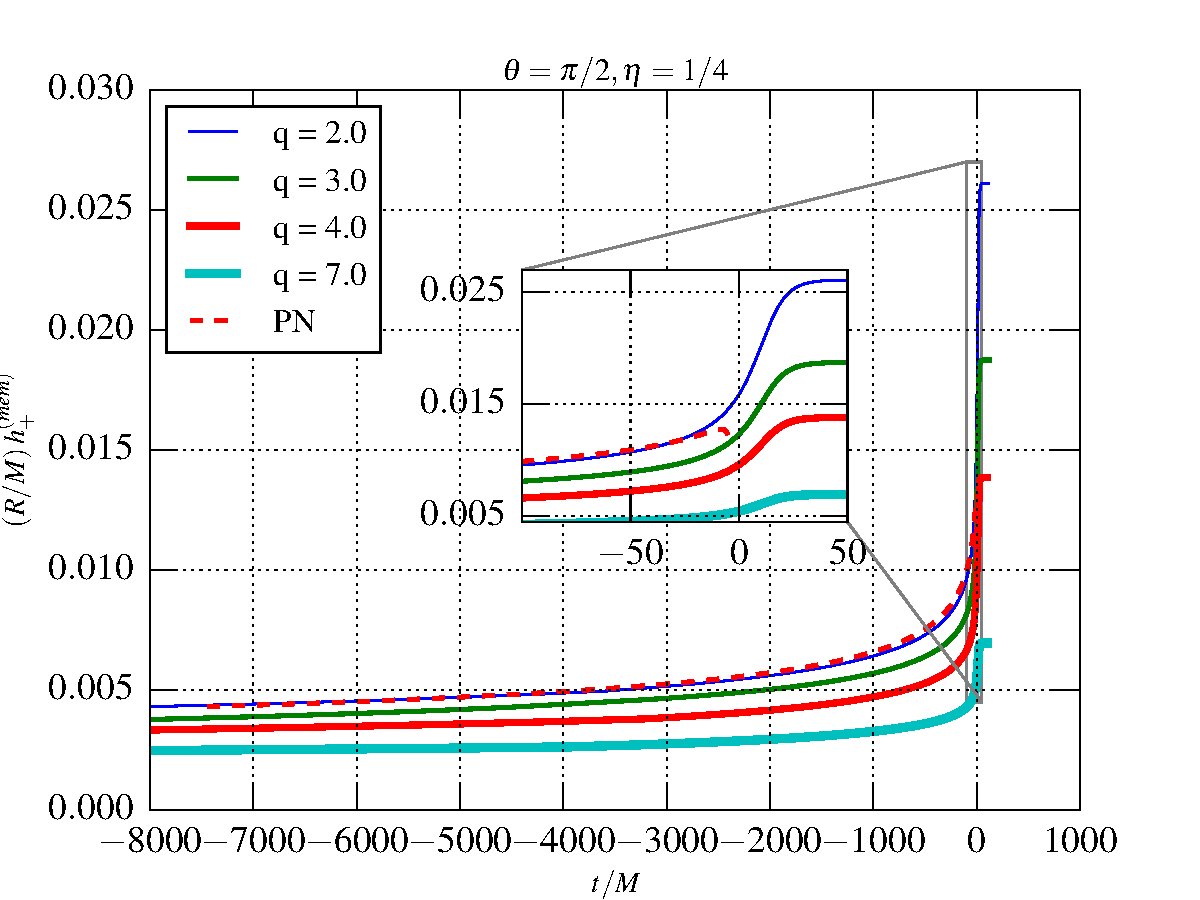
\includegraphics[width=4.0in]{../plots/MemoryPlot_nonSpining/q7.pdf}
\caption{NonSpinning case}
\label{fig:q7}
\end{figure}

\begin{figure}
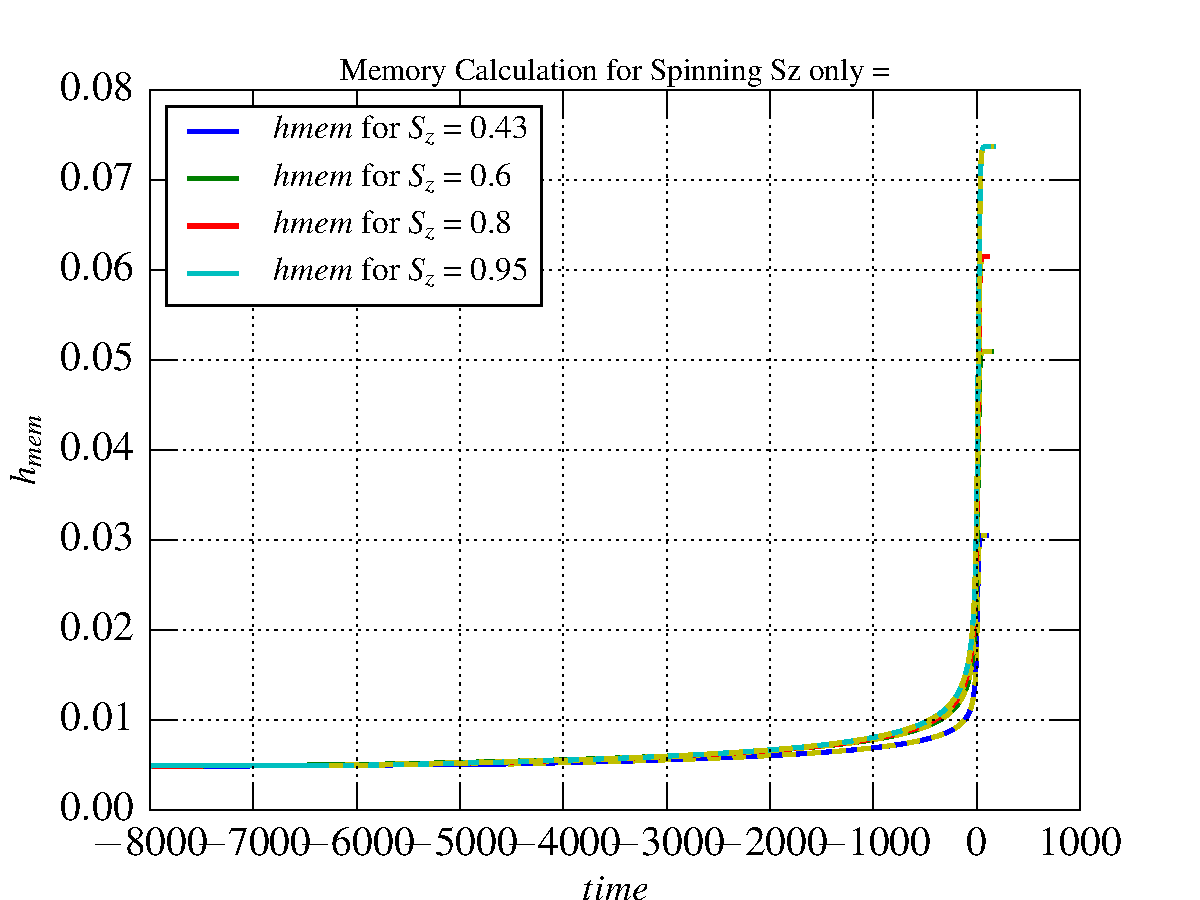
\includegraphics[width=4.0in]{../plots/MemoryPlot_alignedSpin/0p95.pdf}
\caption{NonSpinning case}
\label{fig:0p95}
\end{figure}

\newpage
\appendix 


\bibliography{Spin}

\end{document}
